%!TEX TS-program = xelatex
%!TEX encoding = UTF-8 Unicode

\documentclass[12pt]{article}
\usepackage{geometry}                % See geometry.pdf to learn the layout options. There are lots.
\geometry{a4paper,top=2cm}
\usepackage[parfill]{parskip}    % Activate to begin paragraphs with an empty line rather than an indent
\usepackage{graphicx}
\usepackage{amsmath}
\usepackage{amssymb}
\usepackage{mathtools}
\usepackage{physics}
\newcommand{\be}{\begin{equation}}
\newcommand{\ee}{\end{equation}}
\usepackage[thicklines]{cancel}
\usepackage{url}

\usepackage{fontspec,xltxtra,xunicode}
\defaultfontfeatures{Mapping=tex-text}

\title{Advanced Quantum Mechanics\\Class 11}
%\author{The Author}
\date{September 08, 2022}                                           % Activate to display a given date or no date

\setcounter{section}{5}
\setcounter{subsection}{11}
\setcounter{equation}{127}

\begin{document}
\maketitle

%%% 01 OK
\subsection{Schmidt Decomposition}

A.k.a. Schmidt purification theorem.
It helps to understand entanglement in \emph{pure} systems.
If
\[
|\Psi(1,2)\rangle=|\varphi(1)\rangle|\chi(2)\rangle\left\{\begin{array}{l}|\varphi(1)\rangle \in H_{1} \\ |\chi(2)\rangle \in H_{2}\end{array}\right.
\]
Here the reduced density matrices \(\rho^{(1)}\) and \(\rho^{(2)}\)
are pure (not mixed).

If \(\hat{\rho}^{(1)}\) and \(\hat{\rho}^{(2)}\) corresponding to a pure state
\(|\Psi(1,2)\rangle\) are pure \(\Rightarrow|\Psi(1,2)\rangle\) is a product state
\(\rightarrow\) if \(\hat{\rho}^{(1)}, \hat{\rho^{(2)}}\) are mixed \(\Rightarrow\) entanglement.

\emph{Statement:} For a pure state \(|\Psi(1,2)\rangle\) of a
Tensor-product Hilbert space \(H_{1}\otimes H_{2}\)
of dimensions \(N_{1}\) and \(N_{2}\) respectively,
there exist two orthonormal bases
\(\left\{\varphi_{i}(1) \in H_{1}\right\}\) and 
\(\left\{\chi_{i}(2) \in H_{2}\right\}\) with \(i=1, \cdots, n_{s}\)
where \(n_{s}=\min\left(N_{1}, N_{2}\right)\), such that
\be
|\Psi(1,2)\rangle=\sum_{n=1}^{n_{s}} \sqrt{p_{n}}\left|\varphi_{n}(1) \otimes \chi_{n}(2)\right\rangle
\label{eq:g128}
\ee
\be
0 \leqslant p_{n} \leqslant 1 \text{ and }\sum_{n=1}^{n_{s}} p_{n}^{2}=1
\label{eq:g129}
\ee
$p_{n}$: Schmidt coefficients, \(n_{s}\): Schmidt number

%%% 02 OK

\emph{Proof:}

Suppose first $N_{1} < N_{2}$. Let 
\(\left\{|n\rangle   \in H_{1}\right\}\) and
\(\left\{|\mu\rangle \in H_{2}\right\}\) bases $\to$ 
use Latin indices for $H_1$
and Greek indices for $H_2$.
Then, one can decompose \(|\Psi(1,2)\rangle\) as:
\be
|\Psi(1,2)\rangle=\sum_{n=1}^{N_{1}} \sum_{\mu=1}^{N_{2}} C_{n \mu} | n\otimes \mu\rangle
\label{eq:g130}
\ee
with
\be
\sum_{n=1}^{N_{1}} \sum_{\mu=1}^{N_{2}}\left|C_{n\mu}\right|^{2}=1
\ee
Without loss of generality, one can choose \(\left\{|n\rangle \equiv\left|\varphi_{n}\right\rangle\right\}\)
such that \(\hat{\rho}^{(1)}=\operatorname{Tr}_{2}|\Psi(1,2)\rangle\langle\Psi(1,2)|\) is diagonal:
\be
|\Psi(1,2)\rangle=\sum_{n=1}^{N_{1}} \sum_{\mu=1}^{N_{2}} C_{n \mu}\left|\varphi_{n} \otimes \mu\right\rangle
\label{eq:g132}
\ee
therefore
\begin{align} 
\hat{\rho}^{(1)} 
&=\operatorname{Tr}_{2}|\Psi(1,2)\rangle\langle\Psi(1,2)|\,,
\text{(diagonal)}\nonumber\\ 
&=\sum_{n=1}^{N_{1}} \lambda_{n}\left|\varphi_{n}\right\rangle\left\langle\varphi_{n}\right|%
\label{eq:g133}
\\ 
&=\sum_{n=1}^{N_{1}} \sum_{m=1}^{N_{1}} \sum_{\mu=1}^{N_{2}} C_{n \mu} C_{m \mu}^{*}\left|\varphi_{n}\right\rangle\left\langle\varphi_{m}\right|\tag{$\ref{eq:g133}^\prime$}
\end{align}
Equality of the last two equations implies:
%%% 03 OK
\be
\sum_{\mu=1}^{N_{2}} C_{n\mu} C_{m\mu}^{*} =\lambda_{m} \delta_{nm}
\ee
and
\be
\lambda_{n}=\sum_{\mu=1}^{N_{2}}\left|C_{n \mu}\right|^{2} \rightarrow 0 \leqslant \lambda_{n} \leqslant 1
\ee
Next, change basis in $H_2$ as follows:
\be
|\mu\rangle \rightarrow \sum_{\mu=1}^{N_{2}} C_{n \mu}|\mu\rangle \equiv \sqrt{\lambda_{n}}
\underbrace{\left|\chi_{n}\right\rangle}%
_{\in H_2}
\label{eq:g136}
\ee
\emph{Exercise:} show that $\{\chi_n\}$ are orthonormal:

Use of Eq.~\eqref{eq:g136} into Eq.~\eqref{eq:g132}
\be
\begin{aligned}
|\Psi(1,2)\rangle 
&=\sum_{n=1}^{N_{1}} \sum_{\mu=1}^{N_{2}} C_{n \mu}\left|\varphi_{n} \otimes \mu\right\rangle \\
&=\sum_{n=1}^{N_{1}}\left|\varphi_{n}\right\rangle \sum_{\mu=1}^{N_{2}} C_{n \mu}|\mu\rangle \\
&=\sum_{n=1}^{N_{1}} \sqrt{\lambda_{n}}\left|\varphi_{n}\right\rangle 
\underbrace{\sum_{\mu=1}^{N_{2}} \frac{C_{n\mu}}{\sqrt{\lambda_{n}}}|\mu\rangle}%
_{\ket{\chi_n},\in H_2}\\
&=\sum_{n=1}^{N_{1}} \sqrt{\lambda_{n}}\left|\varphi_{n}\otimes \chi_{n}\right\rangle 
\end{aligned}
\label{eq:g137}
\ee
Identifying $\lambda_n \to p_n$, one obtains Eqs.~\eqref{eq:g128} and \eqref{eq:g129}.

%%% 04 OK

\emph{Note that} we assume $\lambda_n \neq 0$ in Eq.~\eqref{eq:g136}. Is this OK?
Yes, it is OK: we will need Eq.~\eqref{eq:g136} only for $n$
appearing in Eq.~\eqref{eq:g133}.

Given Eq.~\eqref{eq:g137}, what is $\hat{\rho}^{(2)}$?
\be
\begin{aligned}
\hat{\rho}^{(2)}
&=\Tr_1 \op{\Psi(1,2)}{\Psi(1,2)}\\
&=\Tr_1 \left(\sum_{n, m=1}^{N_{1}} \sqrt{p_{n} p_{m}} \op{\varphi_n(1)\chi_n(2)}{\varphi_m(1)\chi_m(2)}\right)\\
&=\sum_{n, m=1}^{N_{1}} \sqrt{p_{n} p_{m}} \op{\chi_n(2)}{\chi_m(2)}
\Tr_1 \underbrace{\op{\varphi_n(1)}{\varphi_m(1)}}_{\delta_{nm}}\\
&=\sum_{n=1}^{N_{1}} p_{n}\op{\chi_n(2)}{\chi_n(2)}
\end{aligned}
\ee

How about if \emph{$N_1 > N_2$}?
Instead of taking \(\left\{|n\rangle \in H_{1}\right\}\) and diagonalizing \(\hat{\rho}^{(1)}\),
one can take \(\left\{|\mu\rangle \in H_{2}\right\}\),  diagonalize \(\hat{\rho}^{(2)}\) and
one would obtain
\be
\hat{\rho}^{(2)}=\sum_{\mu=1}^{N_{2}} p_{\mu}|\chi_{\mu}(2)\rangle\langle \chi_{\mu}(2)|\,,\, 
\hat{\rho}^{(1)}=\sum_{\mu=1}^{N_{2}} p_{\mu}|\varphi_{\mu}(1)\rangle\langle\varphi_{\mu}(1)|
\ee

%%% 05 OK

If \(N_{1}=N_{2}\), it does not matter which reduced density
matrix you choose to diagonalize.

\emph{Some conclusions:}
\begin{enumerate}
\item The summation over the single index in the
Schmidt expansion goes up to the smallest
dimensionality of \(H_{1}\) and \(H_{2}\).
\item The bases \(\left\{\left|\varphi_{n}\right\rangle\right\}\) and \(\left\{\left|\chi_{n}\right\rangle\right\}\) depend on the
pure state \(|\Psi(1,2)\rangle\) being expanded
$\rightarrow$
in general \(|\Psi(1,2)\rangle\) and \(|\Phi(1,2)\rangle\)
in the same \(H_1 \otimes H_2\) cannot both be
expanded in the same \(\left|\varphi_{n} \otimes \chi_{n}\right\rangle\) basis.
\item \(\hat{\rho}^{(1)}\) and \(\hat{\rho}^{(2)}\) have the same spectrum $\rightarrow$
same entanglement entropies, \(S^{(1)}=S^{(2)}\).
\item (\emph{Exercise:}) One can show that 
\be
0 \leqslant S^{(i)}<\ln n_{S}\,,\,i = 1,2 
\ee
\end{enumerate}
Alternative proof of the Schmidt decomposition,
uses the singular value decomposition theorem
of linear algebra.

%%% 06 OK

\emph{``Proof"}: Eq.~\eqref{eq:g130}
\[
\left.
\begin{array}{l}
C=U \Lambda V^{\dagger} \\ 
U: N_{1} \times N_{1} \text { unitary } \\ 
V: N_{2} \times N_{2} \text { unitary } \\
\Lambda: N_{1} \times N_{2} \text { diagonal with }\\
\quad\,\,\,\text{\emph{non-negative} elements}
\end{array}
\right\}
\begin{array}{l}
\text { C nonsquare matrix, cannot } \\ 
\text { be diagonalized } \Rightarrow \text { singular } \\ 
\text { value decomposition theorem. } \\
\text { Look up a good linear algebra book! }
\end{array}
\]
\[
C_{n \mu}=\left(U \Lambda V^{\dagger}\right)_{n \mu}=\sum_{m=1}^{N_{1}} \sum_{\nu=1}^{N_{2}} U_{n m} \Lambda_{m \nu}\left(V^{\dagger}\right)_{\nu \mu}
\]
\textit{e.g.} $N_1 > N_2$:


\begin{center}
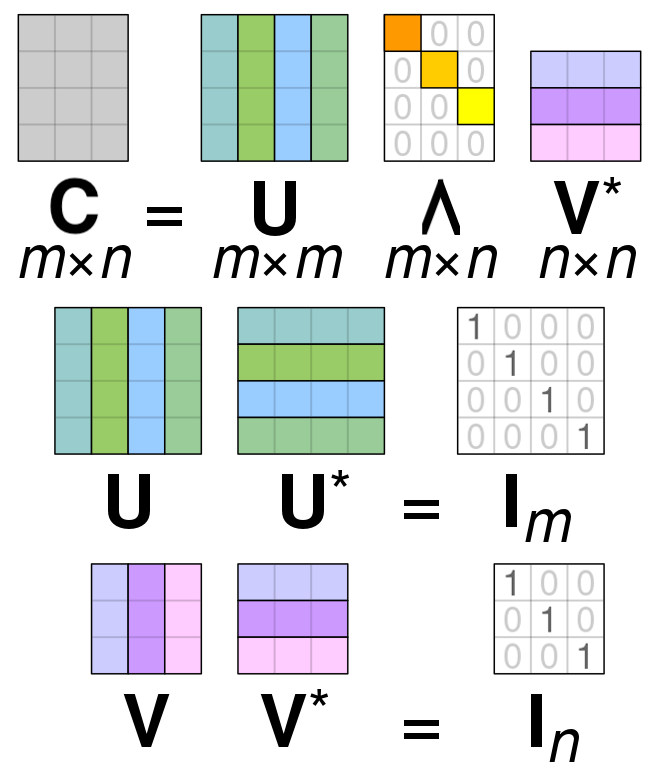
\includegraphics[width=0.6\textwidth]{Figures/SVD.png}
\end{center}


Explicit example: $N_1 = 4, N_2 = 3 \rightarrow$
\be
\begin{pmatrix}
\cdot & \cdot & \cdot\\
\cdot & \cdot & \cdot\\
\cdot & \cdot & \cdot\\
\cdot & \cdot & \cdot
\end{pmatrix} =
\begin{pmatrix}
* & * & * & *\\
* & * & * & *\\
* & * & * & *\\
* & * & * & *
\end{pmatrix}\times
\begin{pmatrix}
\lambda_1 & 0 & 0 \\
0 & \lambda_2 & 0 \\
0 & 0 & \lambda_3 \\
0 & 0 & 0
\end{pmatrix}\times
\begin{pmatrix}
- & - & -\\
- & - & -\\
- & - & -
\end{pmatrix}
\label{eq:g142}
\ee
with $\lambda_i \neq 0, i=1,\ldots, n_s \rightarrow$ smallest between $N_1$ and $N_2$. 

%%% 07 OK
\be
\begin{aligned}
|\Psi(1,2)\rangle
&=\sum_{n, m=1}^{N_{1}} \sum_{\mu,\nu=1}^{N_{2}} U_{n m} \lambda_{m \nu}\left(V^{\dagger}\right)_{\nu \mu} | n \otimes \mu\rangle\\
&=\sum_{m=1}^{N_{1}} \sum_{\nu=1}^{N_{2}} \Lambda_{m \nu}
\underbrace{\left(\sum_{n=1}^{N_{1}}|n\rangle U_{n m}\right)}%
_{\ket{\varphi_m(1)}}
\underbrace{\left(\sum_{\mu=1}^{N_{2}} V_{\nu \mu}^{*}|\mu\rangle\right)}%
_{\ket{\chi_\nu(2)}}\\
&=\sum_{m=1}^{N_{1}} \sum_{\nu=1}^{N_{2}} \Lambda_{m \nu} \left|\varphi_{m}(1) \chi_{\nu}(2)\right\rangle
\end{aligned}
\ee
where $\Lambda_{m \nu}$ has nonzero elements in the diagonal:
$\Lambda_{m \nu} = \lambda_{m}\delta_{m \nu}, m,\nu=1,\ldots,n_s$,
and $n_s = \min(N_1,N_2)$, see Eq.~\eqref{eq:g142}.
Therefore:
\be
\boxed{
|\Psi(1,2)\rangle=\sum_{n=1}^{n_{s}} \lambda_{n}\left|\varphi_{n}(1) \chi_{n}(2)\right\rangle
}
\ee

\emph{Exercise:} show that $\{\ket{\varphi_{n}(1)}\}$ and $\{\ket{\chi_{n}(2)}\}$ are orthonormal.

%%% 08 OK

\subsection{Replica trick}

Computation of the entanglement entropy involves
taking the log of \(\hat{\rho} \Leftarrow\) notoriously difficult
for generic \(\hat{\rho}\)'s.

There exist alternative measures of entanglement
that avoid computing  \(\ln \rho\). One example is
the Rényi entropy:
\be
S_{n}=\frac{1}{1-n} \ln \Tr \hat{\rho}^n, n \text { integer }
\ee
(actually, this is called \emph{n-Rényi} entropy).
Knowing $S_n$, one can imagine that an analytical
continuation of \(n \rightarrow\) integer to real so that
\be
S=\lim _{n \rightarrow 1} S_{n} \rightarrow \text{ replica trick }
\ee

\emph{Proof:}
\begin{enumerate}
\item
\be
\begin{aligned} \Tr \rho^{n} 
&=\Tr\left(\hat{\rho} \hat{\rho}^{n-1}\right)
 =\Tr\left(\hat{\rho} e^{\ln \hat{\rho}^{n-1}}\right) \\ 
&=\Tr\left[\hat{\rho} e^{(n-1) \ln \rho}\right] \end{aligned}
\ee
\item for \(n \rightarrow 1\)
\be
\begin{aligned}
\Tr \hat{\rho}^{n}
&=\Tr[\hat{\rho}(1+(n-1) \ln \hat{\rho})]\\
%%% 09 OK
&=\Tr \hat{\rho}+(n-1) \Tr \hat{\rho} \ln \hat{\rho}\\
&=1+(n-1) \Tr \hat{\rho} \ln \hat{\rho}
\end{aligned}
\ee
\item
\be
\begin{aligned} 
\ln \left(\Tr \hat{\rho}^{n}\right) 
&=\ln [1+(n-1) \Tr \hat{\rho} \ln \hat{\rho}] \\ 
&\stackrel{n\to1}{=}(n-1) \Tr \hat{\rho} \ln \hat{\rho} \end{aligned}
\ee
\item
\be
\lim _{n \rightarrow 1}\left[\frac{1}{1-n}(n-1) \Tr \hat{\rho} \ln \hat{\rho}\right]=\underbrace{-\Tr \hat{\rho} \ln \hat{\rho}}_{S}
\ee
\end{enumerate}
\emph{Note that:}
\be
\lim _{n \rightarrow 1} \frac{1}{1-n} \ln \Tr \hat{\rho}^{n}=\left.\frac{d}{d n} \Tr \rho^{n}\right|_{n=1}
\ee

Yet another entanglement measure is the purity
\(P(\hat{\rho})\) of a state \(\hat{\rho}\) :
\be
P(\hat{\rho})=\Tr \hat{\rho}^{2}
\ee
$\rightarrow$ if the state is pure: $\hat{\rho}^2 = \hat{\rho}$ and $P(\hat{\rho}) = 1$.
\emph{Exercise:} show that
\be
P(\hat{\rho})=\sum_{i} p_{i}^{2},\,0 \leqslant p_{i} \leqslant 1,\, \sum_{i} p_{i}=1
\ee
where the $p_i$ are the eigenvalues of $\hat{\rho}$.

%%% 10 OK

\subsection{Pieces of nomenclature}

Used in many quantum information textbooks.

\emph{Extension} of a reduced \(\hat{\rho}\): If \(\hat{\rho}^{(1)}=\Tr_{2} \hat{\rho}^{(12)}\), then \(\hat{\rho}^{(12)}\) is an extension
of \(\hat{\rho}^{(1)}\). Likewise for \(\hat{\rho}^{(2)}\): \(\hat{\rho}^{(12)}\) is an extension of \(\hat{\rho}^{(2)}\).


\emph{Purification:} Somewhat the reverse of a partial trace;
any mixed state can be seen as the result
of a partial trace in an enlarged Hilbert space.
That is, by adding an auxiliary Hilbert space,
one can always replace mixed states
by pure states in the enlarged space.
In a way, we are appending new degrees of
freedom, not necessarily physical ones
-- these \mbox{d.o.f.} are often called \emph{ancillae}\footnote{%
\textit{Ancillae}: plural of \textit{ancilla} , origin mid \(17^{\text {th }}\) century,
from Latin ``maidservant".%
},
kind of an environment.
In short: purification are pure states that extend mixed states.

%%% 11 OK

\emph{Exercise:} show that two purifications \(|\Psi(1,2)\rangle\) and
\(|\Phi(1,2)\rangle\) in \(H_{1} \otimes H_{2}\) differ by a unitary
transformation.

\emph{Monogamy of entanglement:} entanglement cannot be shared among many systems without restriction.
If two subsystems of a larger system are
entangled, then each of them cannot be
entangled ``very much" with other subsystems
of the larger system.

Example: three spin-1/2 particles (1, 2, 3).
If particles 1 and 2 are in a singlet state,
\(\left(\uparrow_{1} \downarrow_{2}-\downarrow_{1} \uparrow_{2}\right)\), 
then spins 1 and 3 cannot be in a singlet state, 
\(\left(\uparrow_{1} \downarrow_{3}-\downarrow_{1} \uparrow_{3}\right)\).
But why not?
If both (12) and (13) could be
in singlet states, then one could
measure \(\sigma_{x}(2)\) and \(\sigma_{z}(3)\), thereby
revealing the value of the spin of 1
along both axes \((\hat{x}\) and \(\hat{z})\):
this would lead to a violation of the uncertainty principle.

\end{document}